
% Cal Poly Thesis
% 
% based on UC Thesis format
%
% modified by Mark Barry 2/07.
%




\documentclass[12pt]{ucthesis}
\usepackage{ifpdf}

\newif\ifpdf
\ifx\pdfoutput\undefined
    \pdffalse % we are not running PDFLaTeX
\else
\pdfoutput=1 % we are running PDFLaTeX
\pdftrue \fi

\usepackage{url}
\ifpdf

    \usepackage[pdftex]{graphicx}
    % Update title and author below...
    \usepackage[pdftex,plainpages=false,breaklinks=true,colorlinks=true,urlcolor=blue,citecolor=blue,%
                                       linkcolor=blue,bookmarks=true,bookmarksopen=true,%
                                       bookmarksopenlevel=3,pdfstartview=FitV,
                                       pdfauthor={Ryan Verdon},
                                       pdftitle={Getting Biologists to Drop ACID},
                                       pdfkeywords={thesis, masters, cal poly}
                                       ]{hyperref}
    %Options with pdfstartview are FitV, FitB and FitH
    \pdfcompresslevel=1

\else
    \usepackage{graphicx}
\fi

\usepackage{amssymb}
\usepackage{amsmath}
\usepackage[letterpaper]{geometry}
\usepackage[overload]{textcase}
\usepackage{framed}
\usepackage{appendix}
\usepackage{float}


\bibliographystyle{abbrv}

\setlength{\parindent}{0.25in} \setlength{\parskip}{6pt}

\geometry{verbose,nohead,tmargin=1.25in,bmargin=1in,lmargin=1.5in,rmargin=1.3in}

\setcounter{tocdepth}{2}


% Different font in captions (single-spaced, bold) ------------
\newcommand{\captionfonts}{\small\bf\ssp}

\makeatletter  % Allow the use of @ in command names
\long\def\@makecaption#1#2{%
  \vskip\abovecaptionskip
  \sbox\@tempboxa{{\captionfonts #1: #2}}%
  \ifdim \wd\@tempboxa >\hsize
    {\captionfonts #1: #2\par}
  \else
    \hbox to\hsize{\hfil\box\@tempboxa\hfil}%
  \fi
  \vskip\belowcaptionskip}
\makeatother   % Cancel the effect of \makeatletter
% ---------------------------------------




\begin{document}

% Declarations for Front Matter

% Update fields below!
\title{Getting Biologists to Drop ACID}
\author{Ryan Verdon}
\degreemonth{June} \degreeyear{2013} \degree{Master of Science}
\defensemonth{June} \defenseyear{2013}
\numberofmembers{4} \chair{Alex Dekhtyar, Ph.D. (Computer Science)} \othermemberA{Hasmik Gharibyan, Ph.D. (Computer Science)} \othermemberB{Franz Kurfess, Ph.D. (Computer Science)} \othermemberC{Anya Goodman, Ph.D. (Chemistry \& Biochemistry)} \field{Computer Science} \campus{San Luis Obispo}
\copyrightyears{seven}



\maketitle

\begin{frontmatter}

% Custom made for Cal Poly (by Mark Barry, modified by Andrew Tsui).
\copyrightpage

% Custom made for Cal Poly (by Andrew Tsui).
\committeemembershippage

\begin{abstract}

Bioinformatics is the field of science in which biology, computer science, and information technology merge to form a single discipline. The ultimate goal of the field is to enable the discovery of new biological insights as well as to create a global perspective from which unifying principles in biology can be discerned. Bioinformatics involves the analysis of various types of data from multiple sources to create a model of a physical process found in the real world. To do the necessary modeling, data is being piled up in various different biological databases. So far this has worked relatively well. Unfortunately the amount of biological
data being generated is increasing exponentially. Currently, there are several problems with how biological data
is stored. The most depressing issue comes from a survey done by Bry and Kr\"{o}ger in 2003. It found that out of 111 biological databases 40-44 were collections of flat files and 41-42 were relational databases. Both of these types of systems have serious scaling limits. To store all of the biological data in the future, distributed systems are needed.

There exist three types of distributed systems: Consistent Available (CA), Consistent Partition-Tolerant (CP), Available Partition-Tolerant (AP). We argue that AP systems best meet the biologists' requirements for several reasons. First, that the workloads
commonly run on biological databases are reads. So heavy consistency requirements are not needed. Second, the
workloads are non-transactional so there is no need for the ACID constraint commonly found in relational databases. Lastly, availability is important because research should not be hampered by long database queries.

As a proof-of-concept application to show that an AP system works well, we needed a bioinformatics problem
to tackle. Dr. Anya Goodman, a professor in the department of Chemistry and Biochemistry
at Cal Poly, San Luis Obispo, offers a bioinformatics course that covers
several aspects of gene annotation and genomic research. Currently there does not exist a
system in which users can input and save gene annotations and get immediate
feedback regarding their performance. Thus, the Community Genome Annotation Training (\textit{CGAT}) database was born. In our evaluations we compared a MySQL, Couchbase, and MongoDB implementation of the \textit{CGAT}
back end and found that MongoDB (an AP system) performed the best for the
workloads expected on \textit{CGAT}.

\end{abstract}



\begin{acknowledgements}

   Thank you to my "funions", Eriq Augustine and Aldrin Montana, for their work on \textit{CGAT}.
   Thanks to my friends and family for supporting me. Thanks Disneyland for rejuvenating me on
   the last leg of my thesis. Lastly and most importantly thank you Professor Dekthyar for
   being an amazing Professor and adviser.

\end{acknowledgements}


\tableofcontents


\listoftables

\listoffigures

\end{frontmatter}

\pagestyle{plain}




\renewcommand{\baselinestretch}{1.66}


% ------------- Main chapters here --------------------





\chapter{Introduction}
\label{intro}

Bioinformatics is the field of science in which biology, computer science, and information technology merge to form a single discipline~\cite{bioinformatics_factsheet}. The ultimate goal of the field is to enable the discovery of new biological insights as well as to create a global perspective from which unifying principles in biology can be discerned~\cite{bioinformatics_factsheet}. Bioinformatics involves the analysis of various types of data from multiple sources to create a model of a physical process from the real world. To do the necessary modeling, data is being piled up in various biological databases. So far this has worked relatively well. Yet a problem looms on the horizon. According to Dr. Atul Butte, a Stanford professor, the amount of biological data being generated is growing exponentially~\cite{transcript}. He goes on to say:
\begin{quotation}
"So when people think about how fast computers are getting each year, actually the data in life science is growing faster than that. 
In fact, we are going to reach a point where today's computers are just not even going to be able to compute on all the life science data we have~\cite{transcript}."
\end{quotation}

Why should anyone care that biological data will not be analyzed? Breakthroughs in research will take longer to achieve if good data is ignored or thrown out. Although human diseases may not be found in exactly the same form in animals, there may be sufficient data for an animal model that allows researchers to make inferences about the diseases in human beings~\cite{bioinformatics_factsheet}. Bioinformatics promises to rapidly create new knowledge of low-level biological processes. This, in turn, can lead to advances in the diagnosis, treatment, and prevention of many genetic diseases~\cite{bioinformatics_factsheet}. To be able to create new models as fast as possible, all good data gathered by researchers must be analyzed. Currently, the way the data is stored is leading to some problems in the future.


There are three major problems with how the data is stored now.
The first is that the list of biological databases has exploded in number. In 2001 the list only contained 281 databases~\cite{galperin_molecular_2008}. By 2008, the list had over 1000 entries~\cite{galperin_molecular_2008}. That is a massive increase in the sheer number of databases storing data. Each of these databases is usually highly focused and contains  data of a specific type with specific formatting~\cite{biozon}. Unfortunately data stored in different databases can be strongly related and dependent on each other~\cite{biozon}. For a biologist to get the broader context of where a piece of data fits in the grand scheme of things  often requires searches of several databases~\cite{biozon}.

 The next major problem deals with how the data is stored. Bry and Kr\"{o}ger performed a survey in 2003 that looked at 111 biological databases to see how the data was being stored~\cite{bry_computational_2003}. In the survey they found that of the 111 databases they sampled, 40-44 were collections of flat files and 41-42 were implemented as relational databases~\cite{bry_computational_2003}. Both flat files and relational databases have many problems when it comes to storing biological data. 
 
 The last major problem relates to how much data is being stored in each database. This is easy to visualize by looking at a single database. For example, Figure \ref{fig:genbank} shows the growth of GenBank over many years. On the left axis shows how many base pairs were stored in GenBank for any given data on the x-axis. It is easy to see that as sequencing technology improved the amount of genomics data has exploded in volume. 

\begin{figure}[H]
\begin{center}
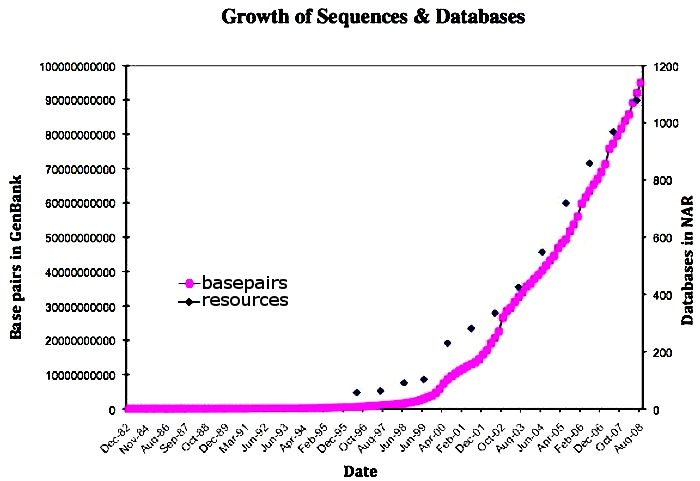
\includegraphics[height=100mm]{genbank_nature_dot_com.jpg}
\captionfonts
\caption[Growth of data inside GenBank]{This figure depicts the amazing growth of GenBank~\cite{nature_graph}.}
\label{fig:genbank}
\end{center}
\end{figure}

As the volume of data increases it will be impossible to house all of the data on a single machine.
To deal with all of the data, distributed systems are needed that manage data across separate
computers or servers.


Recall for a moment how data is stored in computers. There exist three types of distributed systems. This fact comes from a theorem known as Brewer's Theorem, which is often referred to as the CAP Theorem~\cite{brewers_thm}. The theorem presents three attributes of any distributed system, but it states that any distributed shared-data system can have at most two of them. The attributes are consistency, availability, and tolerance to network partitions~\cite{brewers_thm}. Consistency is defined as all nodes in the distributed system seeing the same data at the same time~\cite{brewers_conjecture}. Availability is defined as guaranteeing that every request sees a response about the successfulness of the request~\cite{brewers_conjecture}. Tolerance to network partitions is referring to the ability of a distributed system to lose arbitrarily many messages between two nodes~\cite{brewers_conjecture}. So the theorem leads to the three types of systems: Consistent and Available (CA), Consistent and partition tolerant (CP), Available and partition tolerant (AP). 

CA systems sacrifice the ability to lose arbitrarily many messages between two nodes in order to ensure requests can be immediately dealt with and the system is kept consistent. Usually, in CA systems availability is easily achieved because only one copy of each piece of data is stored. Since there is only one
copy of each piece of data, it is impossible to not be storing the most up-to-date copy. 
The problem arises when a server
in the database goes down. All the data stored on that server is lost until the server is restored. Unlike CA systems, CP systems sacrifice availability to ensure that they can survive one to many server failures. CP systems do this by keeping several copies of every piece of data. To guarantee consistency, on any update or inserts every copy of the data has to be reconciled before a response is sent back. This makes consistency expensive to guarantee. This also leads to a loss of immediate availability. AP systems provide the availability that CP systems can not guarantee, along with the ability to lose arbitrarily many messages between two nodes. AP systems do not provide strong consistency guarantees but allow for great availability by returning the first copy of data found on any query even if that
given copy is old.

Now it is important to go back to the survey done by Bry and Kr\"{o}ger and re-examine their results
using the knowledge gained from the CAP theorem. Recall that of the 111 databases they sampled, 40-44 were collections of flat files and 41-42 were implemented as relational databases~\cite{bry_computational_2003}.
Flat files are a type of system where there is only one copy of each piece of data and the data is stored
in rows like an excel file. Flat files can either be CA or CP systems depending on if the files are stored
on one or several servers. Relational databases, like flat files, depending on the configuration can be
either set up as CA or CP systems. 

So what is wrong with CA and CP systems when it comes to storing biological data? The rapid growth of biological databases is increasing the need for each of the databases to scale up to meet the challenge. Both CA and CP systems have a hard time scaling because they have to provide full consistency on every single node in the cluster. This leads to these systems being slow and inefficient. The full consistency is not needed in many of the biological systems because updates are rare and most of the workload is reads.

Since the strong consistency constraints of CA and CP systems are not needed, there is room for AP
systems to outperform CA and CP systems with biological data. With the knowledge that updates and inserts are rare occurrences, the chances that any node in the cluster has old
data is extremely slim. The ability to respond quickly to any request with what will most likely be the most
up-to-date copy, is extremely beneficial. Also, by having the ability to tolerate network partitions, any
service interruptions can be dealt with as long as the entire cluster does not become unavailable.

As a proof-of-concept application to show that an AP database solution is the best choice, we needed a bioinformatics problem to tackle. Dr. Anya Goodman, a professor in the department of Chemistry and Biochemistry
at Cal Poly, San Luis Obispo, offers a bioinformatics course that covers
several aspects of gene annotation and genomic research. Currently there does not exist a
system in which users can input and save gene annotations and get immediate
feedback regarding their performance. Available gene annotation
software: RepeatMasker, Artemis, and others~\cite{repeatmasker, artemis},is
not designed to provide immediate feedback for users regarding their
performance. Thus, the Community Genome Annotation Training (\textit{CGAT}) database was born. The main goals of \textit{CGAT} are to store and provide feedback on annotations performed by students, professors, and regular people across the world. All of the stored data can be then analyzed to see how effective a community is at creating new knowledge. Why is \textit{CGAT} a good application to show the benefits of an AP system? There are several reasons for this. First, there is a variety of complex data being stored. Second, the workload is read-heavy. Last, the database will need to scale to thousands of users.

The main contributions of this thesis are an argument to support my position that biological databases should move to AP database solutions with the \textit{CGAT} application as a case study. The rest of the thesis is structured as follows. Chapter \ref{previous-work} discusses background information and related work. It is followed by Chapter \ref{dropping_acid} which proposes my argument that AP databases are better equipped to deal with bioinformatics data. Chapter \ref{case-study} examines a proof-of-concept bioinformatics database and shows that an AP database solution is an excellent solution for the requirements. Chapter \ref{evaluation} examines the evaluation of how good an AP solution was for the proof-of-concept database. Lastly, Chapter \ref{conclusions} discusses my contributions, conclusions, and the future work left to be done on \textit{CGAT}.


\chapter{Background and Related Work}
\label{previous-work}

\section{Databases Background}
This section contains all of the necessary background information relating to databases.

\subsection{What is a database?}
A database is an organized collection of data~\cite{database_def}. How the data is organized and accessed is based on the database management software (DBMS) being used. The main tasks of a DBMS is to accept a query, perform some internal processing, and then output the result if any.

\subsection{ACID transaction model}
The ACID transaction model requires very rigid requirements to be used by DBMSs to govern transactions. ACID 
stands for Atomicity, Consistency, Isolation, and Durability constraints. The goal of the ACID transaction model is to provide those constraints on every transaction. Next, it is important to understand what a transaction entails.

\paragraph{Transaction Definition.}
A transaction is a sequence of activities from a particular user that interact with the database~\cite{acid_def}. Activities include querying, inserting, and modifying the database. It is important to note that in the user's environment a transaction is one unit of work, even though the database might have to perform several operations~\cite{acid_def}.

Now that we know what a transaction is, it is important to consider what can go wrong with a transaction and why the ACID transaction model is important for some transactions. Imagine a banking system where users have accounts. In this banking system a common task would be to move money from a users savings account to their checking account. To do this the database must first subtract the amount being transferred from the savings and then add the same amount to the users checking account. Using this example transaction, let us look at several deadly problems.

What would happen if the transaction successfully completed the subtraction from the savings account but could not successfully add to the checking account. Is this an ok situation to happen? NO! In order to prevent users from losing money, the DBMS implements the \textbf{Atomicity} constraint from the ACID transaction model. An atomic transaction is a transaction in which all of the activities in the transaction are run or none of them are~\cite{acid_def}. This prevents the earlier situation from happening. If addition into the checking account cannot occur, the DBMS will undo the change to the savings account and no money will disappear from the users account.

Let us look at another transaction where a user is moving more money from their savings account then they actually have. This would lead to their savings account balance to be a negative value. Any good banking system would require that a balance for a given account be zero or more. Is it ok if the transaction ran and left the balance as a negative value? No! The database required that the balance not be negative. To prevent transactions from leaving the database in an inconsistent state, the DBMS implements the \textbf{Consistency} constraint from the ACID transaction model. A consistent transaction is a transaction that leaves only legal results in the database~\cite{acid_def}. In other words, once a transaction reaches its normal end  it commits only results that are consistent with the database. In our case this would mean not leaving a balance that is negative.

Imagine a scenario in which two separate transactions are running concurrently. The first transaction is moving money from a users savings account to their checking account. The second transaction is applying a fee to any users whose balance across all of their accounts is below a threshold. If the second transaction can see the changes being made in the middle of the first transaction it could improperly charge the user a fee. Is this an ok situation? No! In order to prevent this from happening, the DBMS implements the \textbf{Isolation} constraint of the ACID transaction model. An isolated transaction has its effects on the database hidden from all other concurrently running transactions~\cite{acid_def}.

In another scenario, let us imagine that a transaction has just successfully added money to a user's account. If the database crashed and the results of the transaction are lost, is this ok? No! After a transaction is completed the results must be made permanent. In order to provide this, the DBMS must implement the \textbf{Durability} constraint of the ACID transaction model. A durable transaction is one that is guaranteed to have its results in the database survive any malfunctions of the database, once its results have been committed~\cite{acid_def}.

Now that we have described the definition of the ACID constraints and have looked at why they may be important, let us examine a weaker transaction model that guarantees less strict requirements but has the added benefits of being faster.

\subsection{BASE transaction model}
The BASE (Basically Available, Soft-state, Eventual consistency) transaction model can be summarized as weak consistency, emphasis on availability, best effort, ok to have approximate solutions, optimistic, simpler and easier to adapt~\cite{brewers_thm}. The central basis for the BASE model comes from Brewer's Theorem also known as the CAP Theorem. The CAP Theorem states that any distributed shared-data system can have at most two of the following choices: consistency, availability, and tolerance to network partitions~\cite{brewers_thm}. Consistency is defined as all nodes in the distributed system see the same data at the same time~\cite{brewers_conjecture}. Availability is defined as guaranteeing that every request sees a quick response about the successfulness of the request~\cite{brewers_conjecture}. Tolerance to network partitions is referring to the ability of a distributed system to lose arbitrarily many messages between two nodes~\cite{brewers_conjecture}.

All permutations of the three choices are useful in certain situations. For example, there exist several distributed databases and distributed file systems that use consistency and availability. These systems are generally categorized by several common traits, such as two-phase commit protocols and cache validation protocols~\cite{brewers_thm}. Other distributed databases use consistency and tolerance to network partitions. These databases commonly use pessimistic locking and eliminate minority partitions~\cite{brewers_thm}. Choosing which of the three choices to make involves examining the current problem and choosing a distributed database that makes the assumptions that the situation demands.

Figure \ref{fig:guide_nosql} is a quick visual representation of the CAP theorem. It is important to realize that many of the systems listed in the figure can be configured to be two or more permutations of the CAP theorem. For example, based on the MySQL configuration, it can be either CA or CP depending on if sharding is being used or if it is in a master-slave configuration. Below there are examples given for each of the different types of distributed systems.

\begin{figure}[H]
\begin{center}
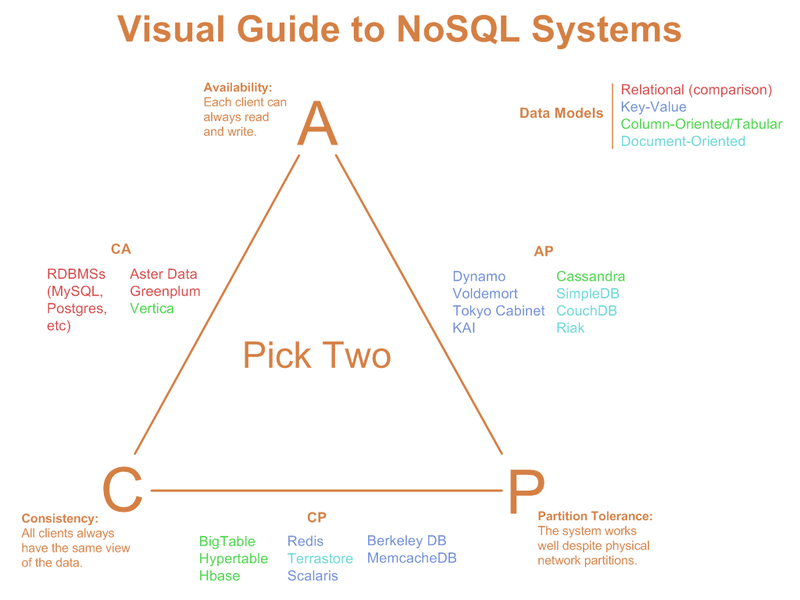
\includegraphics[height=130mm]{cap_theorem.png}
\captionfonts
\caption[Visual guide to the CAP theorem]{This figure depicts visually the meaning of the CAP theorem~\cite{guide_nosql}.}
\label{fig:guide_nosql}
\end{center}
\end{figure}

\subsubsection{Consistent Available Distributed Systems}

Consistent and available distributed systems have the ability to always respond immediately to any request
from clients and the data is kept consistent. The consistency is generally achieved by only keeping one copy
of the data. So there is never any old data lying around on different nodes in the cluster. The ability to 
tolerate network partitions is sacrificed. This is easy to see with the example of a two-node distributed 
database. If one of the nodes goes down, all of the data stored on it is gone with no way to recover it. Availability is easy to provide in CA systems because requests can be serviced as soon as they arrive at the
server. There is no reconciliation process that has to keep all copies of the data consistent because there
is only one copy.

\paragraph{Flat files.}
Flat files are generally plain-text or binary files that contain one record per line. The data in each record is separated by delimiters like commas or tabs. To process a flat file database, a separate program must be written and maintained to correctly perform common create, read, update, delete (CRUD) database procedures. An example flat file database of some NBA members is below.


\begin{framed}
\begin{verbatim}
id    team     last_name
1     Lakers   Howard
2     Lakers   Nash
3     Lakers   Bryant
4     Lakers   Blake
5     Rockets  Brooks
6     Rockets  Jones
7     Rockets  Lin
8     Rockets  Harden
\end{verbatim}
\end{framed}

Flat files are a CA system if there is only one copy of every piece of data kept somewhere in a cluster of servers. 

\subsubsection{Consistent Partition-Tolerant Distributed Systems}

Consistent and partition tolerant systems sacrifice availability to ensure consistency across the cluster
and be able to tolerate partitions. Consistency is achieved by storing a piece of data in several places across
the cluster. CP systems can tolerate partitions because if a node in the cluster becomes unavailable the data
can still be accessed because it is stored elsewhere in the cluster.


\paragraph{Relational databases.}

A relational database defines a set of tables which are represented by the relational data model. In the
relational data model every table has a set of columns which define the attributes of the table. Every table
also has a primary key which is a subset of all of the tables attributes. The primary key ensures that
every row in the table is unique. Tables can relate to other tables by the use of a foreign key. Foreign keys
point to the other table's primary key. There exist several flavors of relational databases. Some of the more common ones include Oracle SQL, MySQL, and Microsoft SQL server.

Generally, for most of the relational database flavors there are several ways to configure them to be either CA or CP. For this example, looking at MySQL, if the cluster is configured to store a complete copy of every table on each server in the cluster, than the relational database is a CP system. This example depicts a CP system because partition tolerance is achieved by storing a copy of every piece of data on every server in the cluster. No matter which node is queried, the same data is returned. If a server goes down there is no effect on the cluster
because the data can still be read because it is copied on every server in the cluster. Availability is lost
since every update, insert, or delete requires changes on every node in the cluster which can take a long time.

\subsubsection{Available Partition-Tolerant Distributed Systems}

Available and partition-tolerant distributed systems sacrifice consistency for increased throughput.
Multiple copies of every piece of data are stored because of the partition-tolerance constraint. To
get the increased throughput, AP systems give up consistency in order to service requests faster. To
guarantee availability, AP systems return the first copy of the data that is found. The given copy might be old
or it might be the most up-to-date. AP systems run a process in the background known as asynchronous updates to ensure that all copies of the data eventually are consistent. 

\paragraph{Domain Name System.}

\begin{figure}[H]
\begin{center}
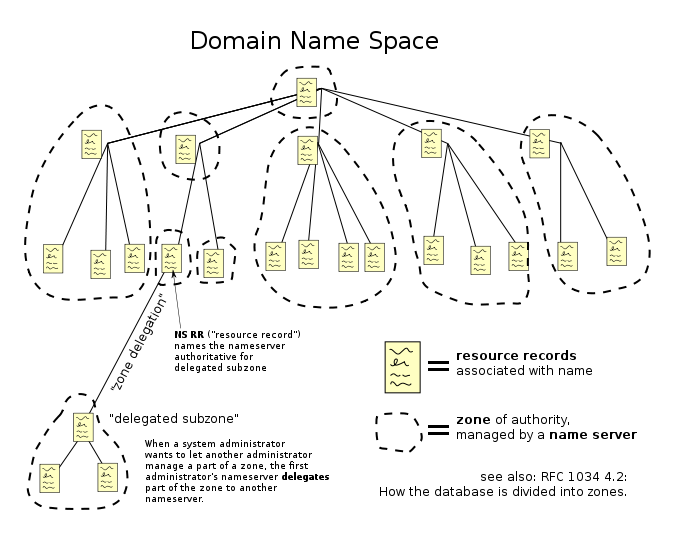
\includegraphics[height=120mm]{dns.png}
\captionfonts
\caption[Example domain name space tree]{This figure depicts an example domain name space tree~\cite{dns}.}
\label{fig:dns}
\end{center}
\end{figure}

The Domain Name System (DNS) is a hierarchical distributed naming system for computers, services, or any resource connected to the Internet or a private network~\cite{dns}. DNS associates several types of information to domain names. Most commonly, DNS translates domain names into IP addresses. DNS is organized
via the Domain Name Space tree. An example Domain Name Space tree is depicted in Figure \ref{fig:dns}. The Domain Name Space is a tree of domain names which starts at the root zone. Each node in the tree contains zero or more resource records which hold information about the domain name. The tree is sub-divided into DNS zones. A DNS zone contains one or more domain names.

It is easy to see that DNS is an AP distributed system by examining how domain names are converted into IPs.
For this example, the fictional domain name www.ryanv.com is located at 192.168.0.1. When someone on the Cal Poly wireless network goes to www.ryanv.com, their browser goes to the Cal Poly DNS server to locate www.ryanv.com. The Cal Poly DNS server does not know about www.ryanv.com because it is not in its DNS zone. So it contacts the root DNS to locate www.ryanv.com. The root server does not know where www.ryanv.com is located but it knows the IP of the .com DNS server. So the Cal Poly DNS server now asks the .com domain name server where www.ryanv.com is. The .com server knows the IP of www.ryanv.com is 192.168.0.1 because the domain name is in its DNS zone. 

With this knowledge of how DNS resolves domain names, let us look at how consistency is not provided. DNS relies
heavily on caching because performing the full domain name resolution is an expensive task. So after the first
time www.ryanv.com is resolved to 192.168.0.1, the Cal Poly domain server will cache the result. Let us imagine
a case where a user goes to www.ryanv.com successfully so the Cal Poly DNS server will cache the IP address.
There is a chance that the IP address of www.ryanv.com will change so while the old IP is cached on the
Cal Poly DNS server, the data will be inconsistent with the real data. 



\subsubsection{CAP theorem revisited}
The main thing to take away from the CAP theorem is that consistency is expensive. Consistency
requires keeping multiple copies of every piece of data up-to-date on all updates, inserts, and deletes.
By not having to keep all copies of the data up-to-date, higher throughput of requests can be maintained.


\subsection{AP Databases Evaluated for the Back End in \textit{CGAT}}

\subsubsection{MongoDB}
MongoDB is a general purpose open-source AP database~\cite{mongodb}. MongoDB has the following major features:
\begin{itemize}
\item Document data model with dynamic schemas
\item Full, flexible index support and rich queries
\item Auto-Sharding for horizontal scalability
\item Built-in replication for high availability
\end{itemize}

MongoDB is a document store type of AP database. Using basic JSON (described in the next section) features, complex data-structure otherwise known as documents can be constructed with nested documents inside~\cite{mongodb}. Using MongoDB's query language, complex queries can be made that can access fields nested deep inside of documents. MongoDB sacrifices consistency when distributed over several servers in order to provide quick querying capabilities.

\subsubsection{Couchbase}
Couchbase is an open-source AP database for interactive web applications and mobile applications~\cite{couchbase}. Couchbase has the following major features:
\begin{itemize}
\item Flexible data model using JSON to represent documents
\item Map-reduce for large aggregate queries
\item Auto-Sharding and other cross cluster cloning capabilities
\item Can create primary and secondary indexes on documents for fast querying
\end{itemize}

Couchbase is a document store type of AP database. At the time the evaluations were run, we were unable to
use common document store database features like being able to query on fields within a document. This is because the document store features were not fully implemented yet. Anyways, key-value
stores provide a \textit{get} and \textit{put} interface. \textit{get}(key) retrieves a value from the given key. \textit{put}(key, value) associates the value with the key provided to \textit{put}.


\subsection{JSON}

JSON (JavaScript Object Notation) is an open standard designed for human-readable data interchange~\cite{json}. JSON is derived from JavaScript. It is used to represent simple data structures with associative arrays known as objects. JSON is often used for serializing and transmitting structured data over the Internet as an alternative to XML.

JSON's basic types include:
\begin{itemize}
\item Number
\item String
\item Boolean
\item Array -- an ordered sequence of values
\item Object -- an unordered collection of key:value pairs with the ':' character separating the key and the value
\item null
\end{itemize}

The example below shows the JSON representation of an object that describes a person. The object contains string fields for first  and last names, a number for age, an object representing the person's address and an array of phone number objects.

\begin{verbatim}
{
    "firstName": "Bob",
    "lastName": "Smith",
    "age": 21,
    "phoneNumbers": [
        {
            "type": "home",
            "number": "(123) 456-7890"
        },
        {
            "type": "mobile",
            "number": "(123) 456-7890"
        }
    ],
    "address": {
        "street": "123 Fake Street",
        "city": "Fake City",
        "state": "CA",
        "zip": 12345
    }
}
\end{verbatim}

\section{Biological Background}
\label{bio-background}
Genomics research attempts to understand information contained in the
\textit{genomes} of various organisms. The genome is the entire DNA sequence
that encodes information and drives all cellular processes in an organism.
However, due to the size of genomes, biologists are only able to sequence
sections, or fragments, of a genome at a time. One or more contiguous fragments
of the genome together form a \textit{contig}, or simply a contiguous sequence
of DNA nucleotides. 

The genome contains several components, or sub-regions,
that have different functions or roles. These components describe in detail how
a genome is decoded to drive cellular processes. \textit{Annotations} -- the
process of linking biological information of the organism to the genome -- are an
important step to being able to relate information learned from the sequence back
to broader understandings of the associated organism and, ideally, related
organisms~\cite{annotation}. 

Again, since the genome is so large, biologists
typically annotate sections of the genome, specifically \textit{genes}. A gene
is a section of the genome that codes for a functional \textit{protein} used
for biological processes inside and outside of the cell. A gene contains
several components, or sub-regions, that have different functions or
roles--\textit{exons}, \textit{introns}, and
others. These components that are located in a gene are some of the most basic but
most important pieces of information that must be annotated in order to be able
to make meaningful biological interpretations from information learned from the
genomic sequence.


%%%%%%%%%%%%%%%%%%%%%%%%%%%%%%%%%%%%%%%%%%%
\chapter{Dropping ACID}
\label{dropping_acid}
I believe that most biological databases should be using AP systems for the back end. This is currently not the case. To attempt to substantiate my position, general observations are presented that come from having examined many biological databases. Then concrete examples of biological databases are shown that match my observations. The example biological databases are evaluated by examining the common tasks performed and by
evaluating the fit of the database back end.

\section{Main Observations}

From my research I have noted four main observations. Each is discussed in turn below.

\subsection{Flat files}
There is a surprising amount of flat file databases still being used by biologists. Some of
the databases are extremely large in size as well. To use the data faster and more efficiently, 
some projects parse the flat file databases into relational databases so that faster querying
can be done.

\subsection{Complex Data}
The data found in biological databases is extremely varied and complex. Types of data can range
from long strands of DNA to images from medical scanners. Not only is the data complex but the relationships
between the data are often complex as well. Frequently, any piece of data can be related to numerous other pieces of data in the same database as well as data in other completely different databases. A good example of
data that is commonly not in the same database are research publications. Normally, when data is uploaded, a
PubMed article ID is stored with it.

With the complex data comes complex metadata. Complex metadata includes who uploaded the data, when it
was uploaded, who touched the data last, when the data was touched last, what changes have been made to the data since it was first uploaded, and more.
 

\subsection{Querying}
From my research, there was very little use of ad-hoc queries. Most of the queries were done through web forms
or APIs set up by the developers. The vast majority of queries were key lookups or index-based lookups. For example, given a PubMed article ID, the system looks up the article. This was an extremely common practice with all types of data. Given the data's ID find the data.

\subsection{Workloads}
The vast majority of the workloads run on the biological databases are reads. Updates and inserts tend to happen in large chunks and happen daily or several times a year.

\section{Example 1: Flybase}
Flybase is the primary biology database on the insect family \textit{Drosophilidae}~\cite{flybase_go}. Biologists examine the fruit fly, \textit{Drosophila},
from the \textit{Drosophilidae} family, to understand the basic principles of genetics~\cite{flybase_board_paper}. Some of the basic principles they are looking for are the nature of genes, genetic linkage, meiotic chromosome segregation, signaling networks and recombination~\cite{flybase_board_paper}. The signaling networks that researchers discovered in fruit flies are now recognized as central factors for major diseases, such as cancer, cardiovascular diseases, and neurological disorders~\cite{flybase_board_paper}. Research on the \textit{Drosophila} has also discovered major processes that affect humans, such as immune responses, stem cells, growth control, learning and memory, neural pathfinding, and synaptic transmission~\cite{flybase_board_paper}. \textit{Drosophila} is also used to model insect vectors of disease, such as malaria, dengue fever, yellow fever, and West Nile Fever~\cite{flybase_board_paper}. Furthermore, the genus \textit{Drosophila} has been used to understand population biology, the molecular basis of speciation, and evolution~\cite{flybase_board_paper}. In short, the fruit fly is very important to biologists! Flybase seeks to be the primary database that stores the genetic information, publications, and terminology of the insect family \textit{Drosophilidae} and allow collaboration among the fruit fly research community. Flybase is found online at \textsf{http://flybase.org}.

\subsection{Database back end}
The Flybase database stores practically all of the data in a single relational database using the Chado schema~\cite{flybase_query_tools}. The Chado schema is used to store biological information from humans to pathogens~\cite{chado}. The data is stored using ontologies. The ontologies are used as a means of typing entities. The schema then uses the types (ontologies) to create a graph that holds the relationships between these types. The schema is partitioned into subschemas; each subschema encapsulates a different biological domain and each is described using different ontologies~\cite{chado}. For example, there is a subschema specifically for publications. Another is for just sequence data. More information on the Chado Schema is found in Appendix \ref{app:chado}.

\subsection{Tasks}
The Flybase website provides a variety of features for the user~\cite{flybase}. The functionality ranges from several implementations of bioinformatics algorithms that can be run on the data in the database, to viewing images of flies. A user can upload papers and genetic data via submission tool, and query the database using several different query tools. The website also includes tools to link pieces of data in the database to other data. Users can also download precomputed data directly from the websites FTP server. The data that can be downloaded includes a recent database dump, genes, alleles, ontology terms, genetic information, and more. Figure \ref{fig:flybase-ss}
shows one of the many query tools found on the Flybase website.

\begin{figure}[H]
\begin{center}
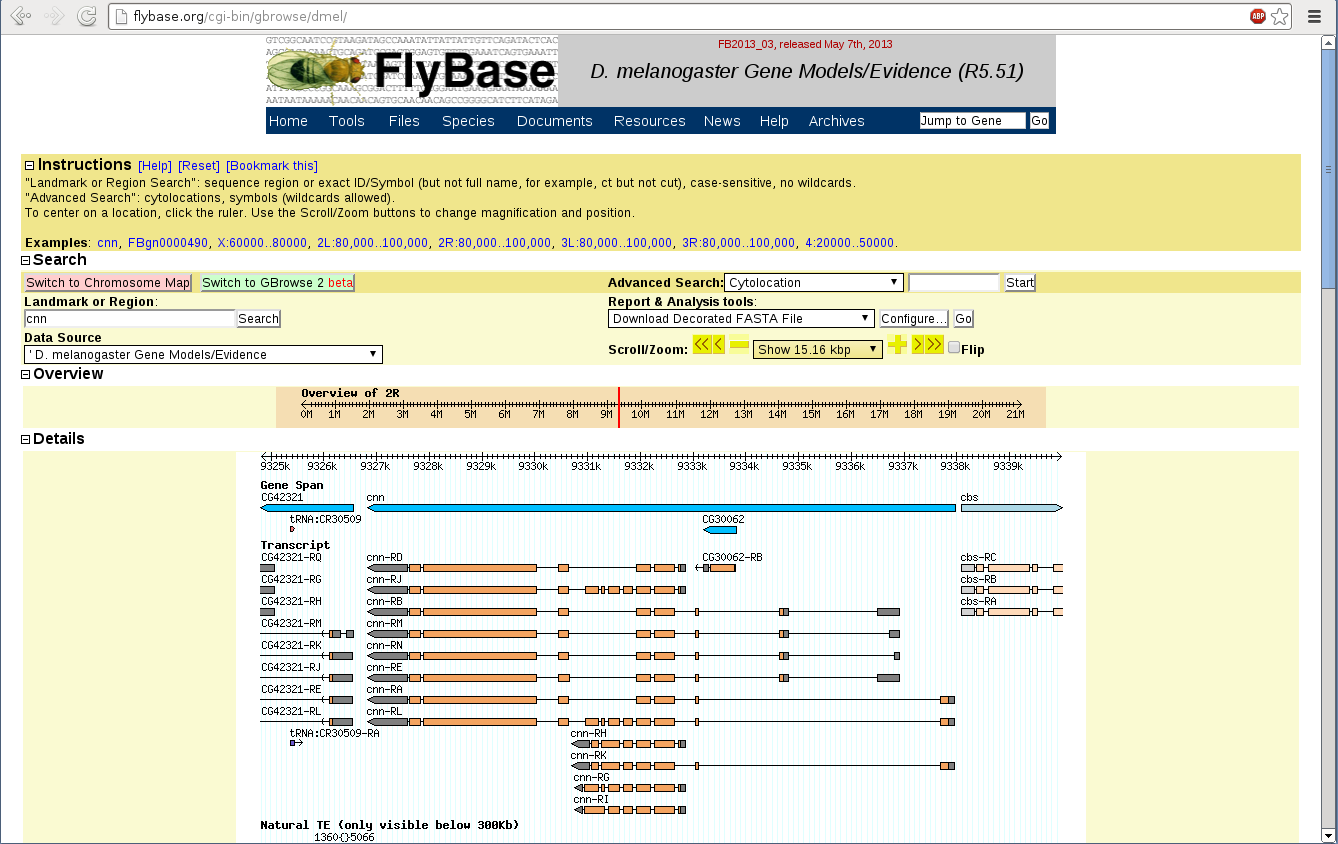
\includegraphics[height=135mm,angle=90]{flybase-screenshot.png}
\captionfonts
\caption[Flybase screenshot]{This figure shows one of the many query tools found on the Flybase website.}
\label{fig:flybase-ss}
\end{center}
\end{figure}

\subsection{Problems}
First of all it is important to examine what type of system the database is running on. The Chado schema
is for relational databases so it is obvious that Flybase is running a relational database. Now depending 
on the configuration being used by the relational database, it can either be running a CA or CP system.

Next we need to examine the nature of data stored in Flybase. The data in Flybase is stored as graphs which
are very similar to objects found in object-oriented programming. In order to store the data, several tables
are used and to get the full graph, many joins must be used.

Not only is the data very object-oriented, the workload that is performed on Flybase does not justify having a CA or CP system. Updates and insertions are rare. The end-users of Flybase are querying from old data for around a month before a big update happens. Therefore, there is no need for the strong consistency guaranteed by the ACID transaction model. By switching to an AP distributed system, Flybase could scale more.

\section{Example 2: GenBank}
GenBank is a comprehensive genomics database that contains DNA sequences for around 260,000 species~\cite{genbank}. The DNA is obtained from submissions by individual laboratories and batch submissions from large-scale sequencing projects (like the whole-genome shotgun and environmental sampling projects). Via the NCBI Entrez retrieval system, the data from GenBank is incorporated with the major DNA and protein sequence databases along with taxonomy, genome, mapping, protein structure and domain information, and the biomedical journal literature via PubMed.

\subsection{Database back end}
The back end for GenBank is a flat file database consisting of 1861 files with an uncompressed size of 594 GB~\cite{genbank_195}. For an example data file see appendix \ref{app:genbank_data_file}.

The data format used in the flat files is called EST which is organized with keywords and their associated descriptions. Every line is considered a record, and the first 10 characters allow for the keyword or sub-keywords. The rest of the line contains the information pertaining to its keyword.
There exist 18 different keywords that make up a possible EST entry. Different keywords define a specific meaning and usage. Some of the keywords are allowed to repeat in a given EST entry, such as the REFERENCE
keyword.

Below is a quick guide to all of the keywords that could show up in an EST entry:
\begin{itemize}
\item The \textbf{LOCUS} field contains information on the GenBank record and a short 
name describing it. Information in the field includes how many base pairs are in the nucleotide snippet, what direction, type of sequence, ACCESSION number (described later), and the date submitted to GenBank.

\item The \textbf{DEFINITION} field provides space for a definition of the sequence.

\item The \textbf{ACCESSION} field has the record's ACCESSION number, as well as any 
ACCESSION numbers related to this record. Every record has a unique ACCESSION number for identifying purposes.

\item The \textbf{VERSION} field contains this record's ACCESSION 
number and a numeric version. 

\item The \textbf{KEYWORDS} field contains all annotated entries via a semicolon separated keywords list.

\item The \textbf{SOURCE} field provides the common name of the organism that the DNA came from.

\item The \textbf{ORGANISIM} field contains the formal scientific name of the SOURCE field along with other taxonomy information.

\item The \textbf{REFERENCE} field allows the record to cite where it came from. 

\item The \textbf{TITLE} field is the full title of the citation from the REFERENCE field.

\item The \textbf{AUTHORS} field lists the authors of the citation in the REFERENCE field.

\item The \textbf{CONSRTM} field allows for a consortium of organizations to be authors rather than every individual in the organizations.

\item The \textbf{JOURNAL} field has the journal name, page number, year, volume of
the citation in the REFERENCE field.

\item The \textbf{REMARK} field specifies the relevance of this citation in the REFERENCE field to this entry.

\item The \textbf{COMMENT} field allows for additional comparisons, comments, and notes.

\item The \textbf{FEATURES} field has the biologically interesting information. For example, how the experiment was performed, where in the genome, and special information of portions of the sequence.

\item The \textbf{ORIGIN} field has the point of origination in the genomic map and how 
the first base of DNA is reported. The ORIGIN field is followed by the DNA sequence data.

\item The \textbf{PUBMED} field is used to reference the PubMed citation database~\cite{pubmed}.

\item The \textbf{MEDLINE} field contains the Medline unique identifier if it exists for this record~\cite{medline}.
\end{itemize}

\subsection{Tasks}
The most common task performed is to display information via the NCBI Entrez retrieval system on a web page in human-readable form. The next most common tasks include daily updates of new sequences and providing major revisions of the database to researchers. These include a lot of updated data. A less common task is removing sequence data for reasons that could include privacy. Figure \ref{fig:genbank-ss} shows the ACCESSION number
CO069431 being retrieved via the NCBI Entrez system.

\begin{figure}[H]
\begin{center}
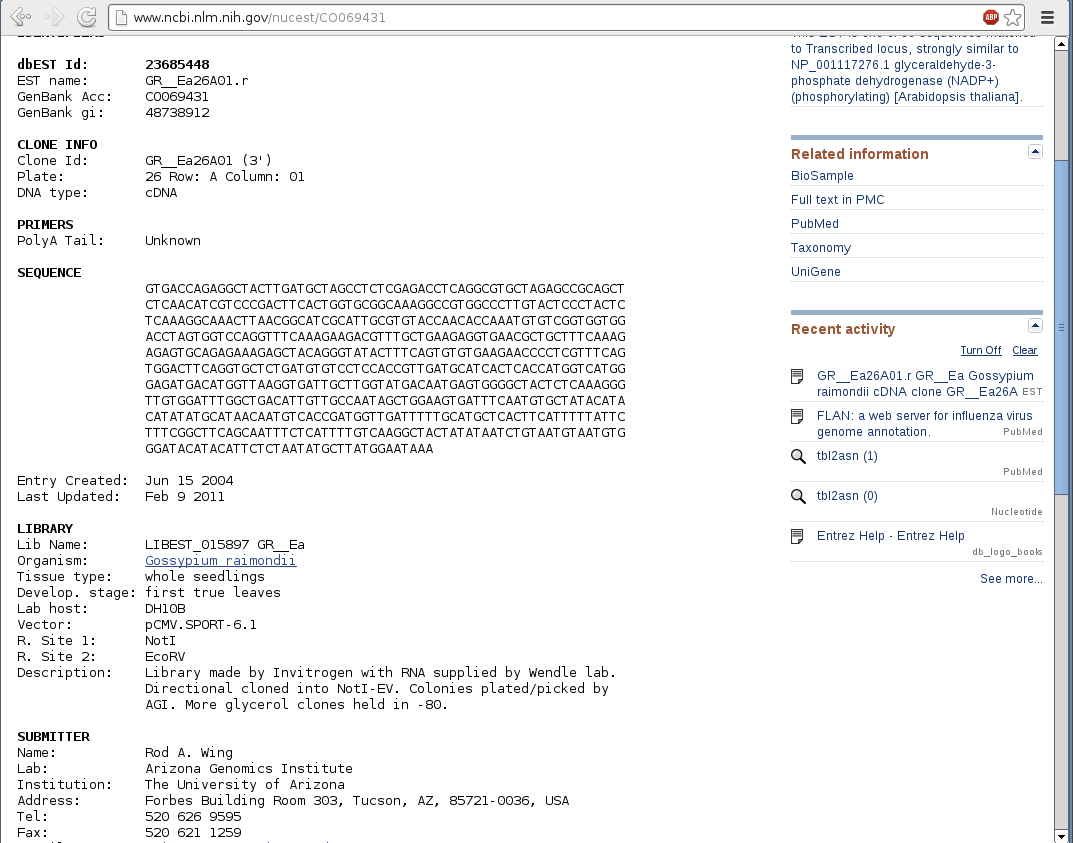
\includegraphics[height=140mm, angle=90]{genbank-screenshot.png}
\captionfonts
\caption[GenBank screenshot]{This figure shows the ACCESSION number CO069431 being retrieved.}
\label{fig:genbank-ss}
\end{center}
\end{figure}

\subsection{Problems}
First, let us examine the system being used by GenBank. We know that GenBank uses a collection of flat files.
We do not know if the files are stored on more than one server. Therefore, GenBank is either using a CA or
CP system to run their flat file database.

Next, let us examine the data being stored in GenBank. GenBank represents the ultimate key-value store. Records consist of all necessary data and have a unique identifier. Queries performed on GenBank are solely based on the unique identifier. So there is no need for any complex querying. Now that we know the data, let us examine the workloads performed by GenBank. Again, like in Flybase, most
of the workload is querying the database for records and updates rarely happen. 

From this I conclude that the database running GenBank does not need to provide consistency. By storing the data in a flat file CA system, all updates must go through GenBank and take up to 24 hours to show up. If GenBank was running an AP system, even with the eventual consistency, updates would not take even close to 24 hours to complete. Therefore, GenBank is a good example of a biological database that should be running an AP system.


\section{Conclusion}
From my research it should be clear that consistency is not needed in most biological databases. First, the workloads are read-heavy. So it would be rare that someone could read inconsistent data. Second, not only are the workloads read-heavy but the queries performed are most often key/index based lookups. Both of these are what AP systems are designed for. Finally, the data and relationships between the data are complex and not
easily represented in the commonly used CA and CP biological databases (flat files and relational databases).
Often trees or graphs need to be used which is hard to represent and quickly query in flat files
and in relational databases.



%%%%%%%%%%%%%%%%%%%%%%%%%%%%%%%%%%%%%%%%%%%%%%%%%%%%%%%%%%
\chapter{Living without ACID}
\label{case-study}

So now that we have seen that AP systems are an excellent choice for biological database back ends,
it is important to examine when AP systems make the most sense. From the previous chapter the following
key principles should be present for an AP system to perform the best when dealing with biological data:

\begin{enumerate}
\item Read-heavy workload
\item No need for strict ACID transactions
\item Complex data/metadata
\item Querying is mostly key/index-based lookups
\end{enumerate}

With these principles in mind, we needed to implement a biological database as a case study.
Thus the Community Genome Annotation Training (\textit{CGAT}) Database was born.

\section{Community Genome Annotation Training (\textit{CGAT}) Database}
\label{cgat}

Dr. Anya Goodman, a professor in the department of Chemistry and Biochemistry
at Cal Poly, San Luis Obispo, offers a bioinformatics course that covers
several aspects of gene annotation and genomic research. Her work is a part of
the \textit{Genomics Education Partnership} (GEP), based at Washington
University in St. Louis~\cite{gep}. GEP is an organization that aims to bring
genomics research to academic institutions, especially undergraduate classes.
This allows undergraduate students to get the opportunity to learn about, and
practice, basic genomic research and, in turn, contribute meaningful work to
the biological research community. However, GEP does not have an existing
system in which users can input and save gene annotations and get immediate
feedback regarding their performance. Similarly, available gene annotation
software -- RepeatMasker, Artemis, and others~\cite{repeatmasker, artemis} -- is
not designed to provide immediate feedback for users regarding their
performance. 

\textit{CGAT} has been built with usability,
simplicity, and efficiency in mind. It is not a feature-rich and data-rich
genome browser like \textit{UCSC genome browser}~~\cite{ucscbrowser},
\textit{Ensembl}~\cite{ensembl}, or \textit{BioViz}~\cite{bioviz}, nor is it
designed to be a replacement for gene annotation software such as
RepeatMasker, Artemis, or any others, in any aspect other than for teaching, or
practicing, gene annotation. Other gene browsers or annotation software offer
many features to accommodate the needs of the biology community, and so tend to
be complex. Gene annotation, while not a trivial task, can be well-serviced by
a simple data model. Ideally, by focusing on a simple data model, \textit{CGAT}
is able to provide a clean, streamlined experience capable of providing users
with a way to view gene annotations made by others or have their gene
annotations reviewed by experts. In particular, \textit{CGAT} strives towards a
Wikipedia-like emphasis on collaboration and openness. \textit{CGAT} stores a wide variety
of data, including huge continuous stands of DNA, user data, collections of users,
help pages with images, annotation data, and more. Each of the types of data are
complex and require nested data-structures to fully describe them.

\section{Problem}

The following main use cases must be implemented.

\begin{enumerate}
\item People should be able to register and join \textit{CGAT}.
\item Users should be able to upload contigs.
\item Users should be able to upload partial/finished annotations for a specific contig.
\item Users should be able to create and join groups.
\item Users should be able to create help pages.
\item Users should be able to get feedback after submitting annotations.
\end{enumerate}

\section{Data}
\textit{CGAT} stores five crucial pieces of information: contigs, annotations,
users, groups, and help pages. Contigs and annotations are biological in nature, while
users, groups, and help pages are data that help manage \textit{CGAT}.

When biologists sequence genomes, they sequence them in overlapping segments
called contigs. A contig, which is a DNA sequence of some length, contains some
number of genes. Biologists record several pieces of information, called
annotations, about genes including coordinates of components of the gene, such
as exons, and meta information about the annotation like who uploaded it and
when it was done, etc.

Groups are another important part of the usefulness of the system. Users of
like minds or research interests can join the same group to receive important
information. Users are a major part of the data and serve as the central hub that connects the
data. Users upload contigs, create annotations, create help pages, and join groups.
There exists the ability to create a help page for each page in \textit{CGAT}. The help
pages help describe and give tips about the page they refer to.

The following sections describe the major types of data found in \textit{CGAT} in more detail.

\subsection{Contigs}
Information stored about contigs includes:

\begin{itemize}
\item A large sequence of DNA nucleotides
\item A name
\item Name of the species the DNA came from
\item A difficulty value
\item Information on who uploaded the contig
\item When the contig was uploaded
\item The status of the contig (test data, active, or practice)
\item Map of isoform names to annotations for the given isoform
\end{itemize}

\subsection{Annotations}
Information stored about annotations includes:

\begin{itemize}
\item The isoform name of the gene being annotated
\item The contig that was annotated
\item Start and stop locations of the gene on the contig
\item The exons of the gene being annotated
\item Whether the annotation was submitted by an expert
\item Whether the annotation was a partial submission or the complete submission
\item Which strand of the DNA the gene was on (3'- 5' or 5'- 3')
\item Who uploaded the annotation
\item Metadata about the annotation -- when it was created, submitted, and last modified
\end{itemize}

\subsection{Users}
Information stored about users includes:

\begin{itemize}
\item First name
\item Last name
\item Login information -- username, password hash and salt
\item Email address
\item The users role -- default user, expert, admin
\item Experienced gained from submitted annotations
\item The users "level" -- level up by gaining experience
\item Metadata information -- date they joined and last time they logged in
\item Past annotation history
\item Annotations that are currently in progress
\end{itemize}

\subsection{Groups}
Information stored about groups includes:

\begin{itemize}
\item The name of the group
\item When the group was created
\item The description of the group
\item The list of users in the group
\end{itemize}

\subsection{Help pages}
Information stored about help pages includes:

\begin{itemize}
\item The page that the document is for
\item The title of the help page
\item The HTML to be displayed on the help page
\item When the help page was created
\item When the help page was last modified
\end{itemize}

\section{Why are CA and CP systems a bad solution for \textit{CGAT}?}
\label{mysql-impl}

Now that we know more about the data being stored in \textit{CGAT}, let us reexamine CA and CP systems
to make sure they are not the best choice for a database back end. 

The first thing to note is the wide variety of data being stored. Data ranges from long strands of DNA to
HTML code. The next thing to remind ourselves about is the workload of \textit{CGAT}. The vast majority of
queries will be reads. Since the majority of the workload is reads, there is no need to ensure consistency on
each node in the cluster. The last major thing to note is that transactions run in \textit{CGAT} are not transactional. Not transactional in the fact that if someone reads data while a transaction is running, nothing 
will be harmed. \textit{CGAT} is not like a banking database where the last example is an extremely bad situation.

Let us also examine the most common choice for web-application database back ends and see that
even relational databases have noticeable problems with the data stored in \textit{CGAT}. Figure \ref{fig:sql-diagram} depicts the ER-diagram for \textit{CGAT}. From the ER-diagram it is easy to see that several issues arise quickly. Getting all of the data about an annotation requires three joins. As the amount of data in those tables increase, that query will be extremely slow. Other issues arise from the fact that sequences in contigs have to be stored as blobs. The size of sequences in contigs can vary from 10k nucleotides to 50k+ nucleotides
so there is no feasible option to use strings to store sequences without wasting lots of space. These
are just some of the issues that would effect scaling with the SQL version of \textit{CGAT}. Taking all
of these issues into account, it is clear that the most common choice for a web-application is not meant for \textit{CGAT}.

\begin{figure}[H]
\begin{center}
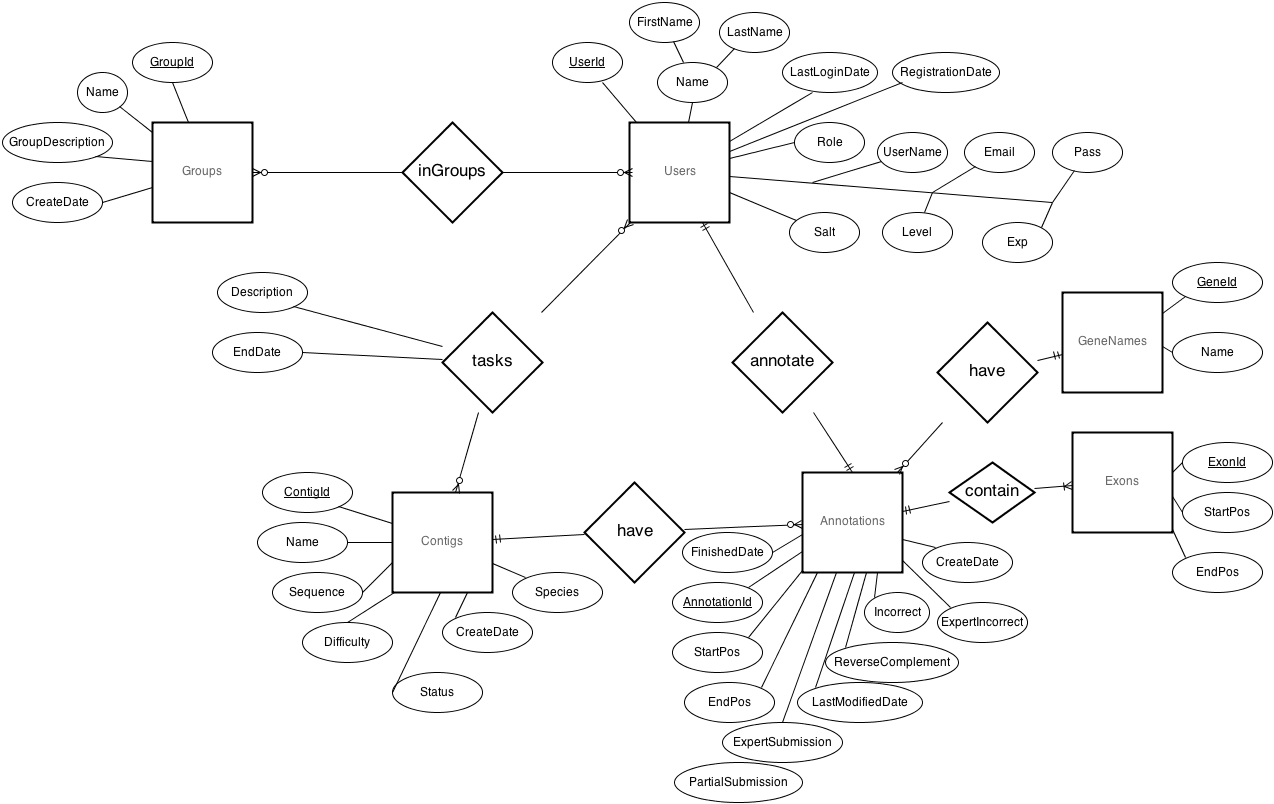
\includegraphics[height=120mm,angle=90]{er-diagram.png}
\captionfonts
\caption[ER Diagram of \textit{CGAT}]{ER Diagram for the SQL version of \textit{CGAT}.}
\label{fig:sql-diagram}
\end{center}
\end{figure}

\section{Implementation}
\label{cgat-implementation}
\textit{CGAT} uses a standard LAMP (Linux Apache MySQL PHP) stack with the ability to replace MySQL with any AP system. As long as it is possible for a database to implement the needed API calls, any system
can be used. The implementation of \textit{CGAT} started in CSC 560 in Fall 2012. We first implemented
a Couchbase back end for \textit{CGAT} because of how the course was structured and an assignment. After
an evaluation comparing a MySQL back end for \textit{CGAT} and our Couchbase version, we saw that Couchbase
performed terrible for read-heavy workloads even though it was set up as an AP system.

Not being extremely fast for read-heavy workloads meant that Couchbase was a bad choice for \textit{CGAT}.
We examined why Couchbase was bad and saw that we needed more than a key-value store to perform better than
MySQL. So we then created a MongoDB back end which is still being used in
\textit{CGAT} today. In what follows, we describe the MongoDB implementation. Then we go over how the Couchbase
back end differed from the MongoDB implementation.

\subsection{Website Back end}
The website back end of the system consists of a PHP server connecting to a MongoDB database.
We do not use any templating systems. We chose PHP for the back end because we did not require most of the functionality of a templating system, and we wanted a simple system that can be easily understood when passed off to the next generation.

PHP and MongoDB work together very nicely and MongoDB's PHP connector is fully featured~\cite{phpMongo}.

\subsubsection{Database Schema}
Although we use MongoDB, which does not enforce a specific schema, by convention we enforce a schema on our documents. MongoDB uses BSON (Binary JSON). BSON is an extended JSON format that supports additional types like a datetimes~\cite{bson}. MongoDB stores documents in collections. We had a separate collection for
each type of document. Figures \ref{fig:contig-ex}, \ref{fig:group-ex}, \ref{fig:annotation-ex}, \ref{fig:user-ex}, \ref{fig:help-ex} depict the BSON version of each type of document found in \textit{CGAT}.


\begin{figure}[H]
\begin{center}
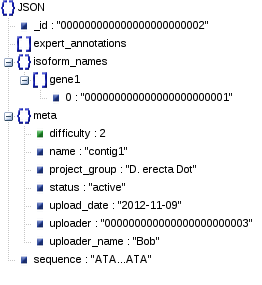
\includegraphics[height=100mm]{contig.png}
\captionfonts
\caption[Contig Document]{Example contig document.}
\label{fig:contig-ex}
\end{center}
\end{figure}

\begin{figure}[H]
\begin{center}
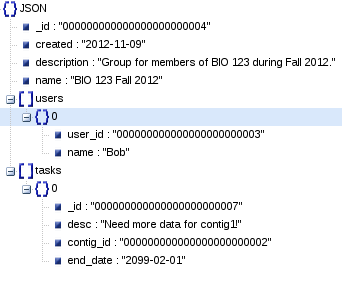
\includegraphics[height=80mm]{group.png}
\captionfonts
\caption[Group Document]{Example group document.}
\label{fig:group-ex}
\end{center}
\end{figure}

\begin{figure}[H]
\begin{center}
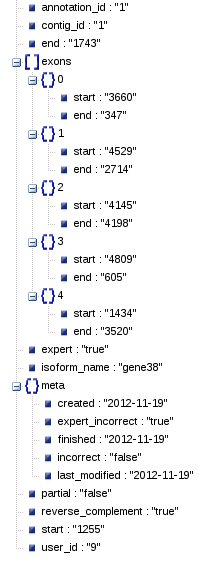
\includegraphics[height=170mm]{annotation.png}
\captionfonts
\caption[Annotation Document]{Example annotation document.}
\label{fig:annotation-ex}
\end{center}
\end{figure}

\begin{figure}[H]
\begin{center}
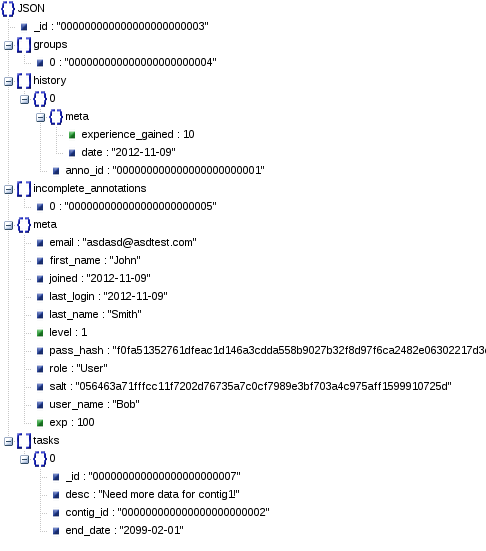
\includegraphics[height=150mm]{user.png}
\captionfonts
\caption[User Document]{Example user document.}
\label{fig:user-ex}
\end{center}
\end{figure}

\begin{figure}[H]
\begin{center}
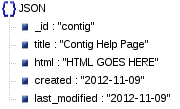
\includegraphics[height=35mm]{help.png}
\captionfonts
\caption[Help Page Document]{Example help page document.}
\label{fig:help-ex}
\end{center}
\end{figure}


\subsubsection{API}
\textit{CGAT} is an entirely API-driven product. The API is central to all the behavior.
The API supplies \textbf{all} the information that is displayed in the UI.
This is a very important design choice. Having the API be the sole data provider and manipulator for the system
means that all functionality can be programmatically provided and different applications can present the same
functionality with a different UI. Thus the programmers working at GEP can extend current genome browsers to store data in \textit{CGAT}.

The API accepts GET and PUT requests (depending on the action) and will always return a JSON response.
Having an API is why switching out the database back end is extremely easy. 
As long as any database provides a PHP driver, it can be used in \textit{CGAT}. To switch out
the database, all that needs to happen is to implement the API calls in the new database,s PHP driver.
The current API supports 23 different calls, 9 GET requests, and 14 POST actions.

\paragraph{GET Requests.}
Most get requests do not require the user to be logged in. Table \ref{tab:get_requests} lists
the get requests found in the \textit{CGAT} API.

\begin{table}[H]
   \centering
      \begin{tabular}{| l | p{10cm} |}
         \hline
            {\textbf{Get Request Name}} &
            {\textbf{Information}} \\
         \hline
            administration\_info & Provides the user with meta information that the user would need to perform administrative tasks such as creating a group or assigning a task. \\
         \hline
            annotation           & Provide the user with information about a specified annotation.  \\
         \hline
            contig  & Get information about a specific contig.  \\
         \hline
            claim      & Get all contig information in a specific project group. Used for claiming new contigs to annotate.  \\
         \hline
            gene           & Get information about a specific gene. \\
         \hline
            get\_feedback           & Get feedback for a specific annotation. \\
         \hline
            group              & Get information about a specific group. \\
         \hline
            help              & Get help information on a specific topic. \\
         \hline
            user\_profile              & Get the profile information about a specific user. If the user is logged in and requests information about themselves, more information is provided. \\
         \hline
      \end{tabular}
      \caption{Table of the get requests found in the \textit{CGAT} API.}
      \label{tab:get_requests}
\end{table}

\paragraph{POST Actions.}
Most POST actions require that the user is logged in. Table \ref{tab:post_requests} lists
the post requests found in the \textit{CGAT} API.


\begin{table}[H]
   \centering
      \begin{tabular}{| l | p{10cm} |}
         \hline
            {\textbf{Post Request Name}} &
            {\textbf{Information}} \\
         \hline
            assign\_task & Ask a group of people to perform an annotation. \\
         \hline
             cancel\_notification  & Clear a notification from a user. \\
         \hline
            create\_annotation & Create a new annotation of a contig. \\
         \hline
            create\_group & Create a group. \\
         \hline
            join\_group & Join a group. \\
         \hline
            leave\_group &  Leave a group. \\
         \hline
            login & Login. \\
         \hline
            logout           & Logout.  \\
         \hline
            parse\_fasta  & Upload a FASTA file to the server, parse the contents, and return the parsed structure.  \\
         \hline
            register      & Register a new user.  \\
         \hline
            save\_annotation           & Save a work-in-progress annotation. \\
         \hline
            set\_help              & Upload a help page. \\
         \hline
            submit\_annotation              & Submit a finalized annotation. \\
         \hline
            upload\_contig              & Upload a contig into \textit{CGAT}. \\
         \hline
      \end{tabular}
      \caption{Table of the post requests found in the \textit{CGAT} API.}
      \label{tab:post_requests}
\end{table}

\subsection{Front end}
\textit{CGAT}'s front end uses standard web technologies (HTML, Javascript, and CSS).
\textit{CGAT} uses many HTML5/CSS3 features such as transforms and pseudo-elements.
Because the entire system is API based, the front end heavily relies on asynchronous fetches (AJAX).

\subsection{Common Workloads}
\label{common-work}
This section contains the most common workloads run on \textit{CGAT}. By far the most common
are the first three workloads which are read-heavy. Each workload is discussed below in turn.

\subsubsection{Profile View}
The first thing that all users will do in \textit{CGAT} (ideally) is log in.
When a user logs into \textit{CGAT}, the user is directed to their profile
view which contains all groups they are a member of, all completed
annotations they have submitted, partial annotations that have been saved, and
all tasks they have assigned. This is a workload that is likely to see many
additions in the future as it serves as the first and foremost view of the
system for the user. This means that any information that should be accessible
-- including when a forum system is integrated into \textit{CGAT} -- will find
a place on the user's profile.

This workload is clearly a read-heavy workload that entails no disk writes at
all. Important to note though, this use case may constantly be increasing
(should constantly be increasing for a successful system) and so the may increase quite a bit, and whenever new features are added,
there is a potential for a spike in workload.

\subsubsection{Task Assignment}
In \textit{CGAT} it must be possible to request a group of users to annotate
new or updated contigs. The frequency of this use case is dependent on the
adoption of \textit{CGAT} -- the more species \textit{CGAT} supports, the more
frequent this use case will be. More specifically, the relevant entities in the
\textit{CGAT} schema are \textit{users}, \textit{contigs}, and \textit{groups}.
Since a task embodies a request for a group $G$ to annotate a contig $C$, every
user $U$ in $G$ receives a notification including a description of $C$ and a
message requesting that it be annotated. A task can be assigned to any number
of groups. Since tasks are assigned to groups that have some vested interest in
the species or specific contig that has been updated or added, there may be
many groups that a task should be assigned to. Additionally, as more species
are supported by \textit{CGAT} or more users join \textit{CGAT}, more users
will receive notifications of tasks and so there are multiple ways in which
this workload must be scalable.

This workload is read-heavy since group, contigs, and users must be queried before
adding tasks.

\subsubsection{Annotation Publication}
Annotations are the core focus of \textit{CGAT}. Every user is going to be
uploading some annotations. Hopefully they should be uploading many annotations. Especially
since \textit{CGAT} defines an annotation to be information about a gene
isoform, variation, on a contig, even annotating a single gene will yield several
annotations in \textit{CGAT}. Additionally, when an annotation is submitted,
the annotation is marked as complete, the user and annotation are then
assigned a certain amount of experience -- the user gains experience towards
his or her total, the annotation gains experience and serves as a history of the
user's experience.

This is a mostly read-heavy workload with some writes. It is mostly read-heavy in the
sense that it must eventually do some writing
by updating a user and the annotation that the user completed.
However, it also has a lot of reads in the sense that the contig, for which the
annotation is being submitted, and the user have to be queried to determine the amount of experience
that submitting the annotation yields for the user. 

\subsubsection{Group Modification}
Group membership is likely the second most stable of the workloads. This is ``stable''
because the majority of users will only join groups, and leaving groups will
likely be relatively rare. This workload will only ever be as bad as how many
users join at any one time -- once a user registers for \textit{CGAT} and has
joined some groups, the user is unlikely to join or leave groups, and so this workload
poses almost no scalability problems. Although, despite this, there will
be spikes that coincide with academic schedules, as groups will be created and
populated for each new class that uses \textit{CGAT}.

This workload is the most balanced of the workloads. Generally speaking, when a user joins a
group, then there is only the addition of a user id in the group document and a 
group id in the user's document. And when a user leaves a group, then
the previous changes are undone by removing the user id and group id from their respective documents.

\subsubsection{Contig Uploads}
Contig uploads is the most stable workload when the manual, or user, use case
is considered. Although, there will be large spikes of activity when/if the
reference genome for a species is updated,requiring \textit{CGAT} to update
any and all of the contigs relevant to the genome. However, reference genomes
are updated very infrequently and contigs will never be removed from
\textit{CGAT}.

This workload is write-heavy because it requires no reads -- the workload is for
uploading data, not downloading data.

\subsection{Couchbase Implementation}
The Couchbase back end slightly differed from the MongoDB version. The Couchbase implementation stored
the same JSON documents as the MongoDB implementation. The only difference was how documents were accessed.
In Couchbase a user document for the user with the ID of 1 was stored with the key "users-1". Same
idea for the group document with the ID of 5 ("groups-5"). Whenever a document that was being manipulated
had a reference to another document, the way to query for the referenced document was by hyphenating the type of document with the ID being searched for.

\chapter{Evaluation}
\label{evaluation}

Traditional web applications are almost always backed by a relational database.
Since \textit{CGAT} is being backed by an AP system it is important to consider the performance ramifications.
The main goal of the evaluation is to determine how an AP implementation compares to a traditional back end like MySQL. If my argument is correct, the AP implementations should perform better for read-heavy workloads. For the evaluation we compared a CP configuration of MySQL, an AP configuration of Couchbase and an AP configuration of MongoDB.


\section{Experiment Design}\label{sec:design}
To evaluate the performance of the different implementations, we generated around 400MB
of data that was used by each system\footnote{The data models used are depicted in Chapter \ref{case-study}.}.
We then created a set of six experiments to run. Five came from common workloads
found in \textit{CGAT}. Recall from Section \ref{common-work} that these are
profile view, publishing annotations, group modification, contig upload, and task assignment.
The final experiment was a contrived one designed to test the performance on each cluster by repeatedly writing and
reading from the same object. Our major metrics are write performance, read
performance, and time-delay between writes and reads of the same data.

For our experiments, we are using a total of five EC2 instances from the Amazon
Web Services cloud offering. For all of the implementations, four servers were used
for the database cluster while the fifth was used for running our workload harness.
The MySQL system is setup with one master server for writes and three
slave servers that replicate all of the masters data. Similarly, the MongoDB system
was setup with one master for writes and three replicas for read performance. 
The Couchbase
system was configured in a way where each server handled a subset of the data. The main tasks of the
workload harness was to define how many times a workload would run and which
workloads to run. In our case, workloads represent a certain task or use case
in \textit{CGAT}. For example, retrieving data that is displayed on
a user's profile. In our system, a workload knows how to do its job in all of the implementations.
As each workload is run, the workload harness
records important statistics. These include the length of time the workload
took to complete, the min and max completion times of an individual query or
insertion, and the standard deviations of individual runs.

\subsection{Data}
Our data models have four crucial pieces of information: contigs, annotations,
users, and groups. We chose to not use help pages in our experiments because they did
not show up in the common workloads.

\subsubsection{MySQL}
Our data model in SQL consists of eight relational tables. An ER-diagram of the tables is depicted in Figure
\ref{fig:sql-diagram} from Section \ref{mysql-impl}. In the tests we also added an additional table for the last experiment that tests reading and writing from the same object. The CREATE TABLE statements are located in
Appendix \ref{app:sql}.


\subsubsection{Couchbase and MongoDB}
All of the data in Couchbase and MongoDB is represented in JSON.
 We used four JSON objects
which are shown in Figures \ref{fig:contig-ex}, \ref{fig:annotation-ex},
\ref{fig:user-ex}, and \ref{fig:group-ex} in Section
\ref{cgat-implementation}. All of same information from the MySQL tables is
represented in these JSON objects. We take advantage of nested objects to
reduce as much subsequent requerying of the database as possible.

\begin{table}[t]
   \centering
      \begin{tabular}{| l | c | c | c | c |}
         \hline
            {\textbf{Workload}} &
            {\textbf{MySQL}} &
            {\textbf{Couchbase}} &
            {\textbf{MongoDB}}\\
         \hline
            Task Assignment         & 39325189ms & 157431049ms\footnotemark{} & 5327456ms\\
         \hline
            Profile View            & 2908257ms & 7008818ms & 165409ms\\
         \hline
            Annotation Publication  & 510837ms & 1830064ms & 324601ms\\
         \hline
            Group Modification      & 316673ms & 9086304ms & 1322606ms\\
         \hline
            Contig Upload           & 119892ms & 20133ms & 57124ms \\
         \hline
            Read/Write              & 103808ms & 58581ms & 152268ms \\
         \hline
      \end{tabular}
      \caption{Comparison of runtimes in ms for the different workloads.
               Each workload was run for 100000 iterations.}
      \label{tab:workload_perf}
\end{table}
%footnote text has to be separate from the mark because the table is floating
%and so if you just use the usual '\footnote{}' then the mark shows up in the
%document but not the text. awkies...
\footnotetext{Task assignment never actually completed. The number reported is the
approximate length of time spent running the workload before
giving up. Explanation provided in Section \ref{sec:eval}}

\section{Workloads}\label{sec:workload}
The core unit of work that we used to compare performance was called a \textit{workload}.
Unfortunately, due to time constraints we were
unable to do multiple runs of any one workload, however, due to our environment
and machines, there should be minimal fluctuations in any given run time for a
workload.

The workloads we are running include the five most common workloads in \textit{CGAT}. 
Recall from Section \ref{common-work} that these are profile view,
publishing annotations, group modification, contig upload, and task assignment.
The last workload we ran is discussed below.

\subsection{Read/Write Performance}
This is a test workload to examine the performance of writing and reading from
the same object in succession. This is a naive, balanced workload with even numbers
of read and writes.

\section{Implementation}\label{sec:implementation}
Our experiment was implemented in Java. To do the MySQL portion of
the workload, we used the MySQL JDBC driver. For the Couchbase portion we used
the official Couchbase Java library from their website. Finally, for the MongoDB portion
we used the official MongoDB Java driver.

\begin{table}[t]
   \centering
      \begin{tabular}{| l | c | c | c |}
         \hline
            \multicolumn{4}{|c|}{{\textbf{MySQL read/write performance}}} \\
         \hline
            & \textbf{RAW} & \textbf{WAR} & \textbf{combined} \\
         \hline
            Min (ms) & 0 & 0 & 0 \\
         \hline
            Max (ms) & 25 & 70 & 70 \\
         \hline
            Mean (ms) & 0.473 & 0.558 & 0.516 \\
         \hline
            Median (ms) & 0 & 1 & 0 \\
         \hline
            Standard Deviation (ms) & 0.685 & 0.859 & 0.778 \\
         \hline
      \end{tabular}
      \caption{Comparison of reads and writes to the same object in MySQL.}
      \label{tab:sql_perf}
\end{table}

\begin{table}[t]
   \centering
      \begin{tabular}{| l | c | c | c |}
         \hline
            \multicolumn{4}{|c|}{{\textbf{Couchbase read/write performance}}} \\
         \hline
            & \textbf{RAW} & \textbf{WAR} & \textbf{combined} \\
         \hline
            Min (ms) & 0 & 0 & 0 \\
         \hline
            Max (ms) & 71 & 48 & 71 \\
         \hline
            Mean (ms) & 0.562 & 0.017 & 0.290 \\
         \hline
            Median (ms) & 1 & 0 & 0 \\
         \hline
            Standard Deviation (ms) & 0.859 & 0.213 & 0.682 \\
         \hline
      \end{tabular}
      \caption{Comparison of reads and writes to the same object in Couchbase}
      \label{tab:couch_perf}
\end{table}

\begin{table}[t]
   \centering
      \begin{tabular}{| l | c | c | c |}
         \hline
            \multicolumn{4}{|c|}{{\textbf{MongoDB read/write performance}}} \\
         \hline
            & \textbf{RAW} & \textbf{WAR} & \textbf{combined} \\
         \hline
            Min (ms) & 1 & 0 & 0 \\
         \hline
            Max (ms) & 11 & 1 & 11 \\
         \hline
            Mean (ms) & 1.491 & 0.027 & 0.759 \\
         \hline
            Median (ms) & 1 & 0 & 1 \\
         \hline
            Standard Deviation (ms) & 0.514 & 0.162 & 0.826 \\
         \hline
      \end{tabular}
      \caption{Comparison of reads and writes to the same object in MongoDB.}
      \label{tab:mongo_perf}
\end{table}

\section{Evaluation}\label{sec:eval}
In this section we discuss the results for each workload in turn. As a general
note, each workload was ran $N$ number of times.
While we initially planned for $N$ to be the same for each workload
($N=100000$), the ContigUpload workload ran into memory constraints of the
EC2 machine running our queries. This caused us to reduce the number of times
the task was repeated ($N=10000$) for the ContigUpload workload.
Additionally, the TaskAssignment workload never completed on Couchbase. The
runtime reported for this workload was the amount of time the TaskAssignment
workload was running. We had waited approximately 45 hours before finally killing
the workload harness.

\subsection{Task Assignment}
From Table \ref{tab:workload_perf}, it is obvious that MongoDB significantly
outperforms both MySQL and Couchbase for the TaskAssignment workload. We think this is due to
the read-heavy nature of this workload. MySQL performed better
than Couchbase because MySQL's data model allows
simple ad-hoc query to find necessary values prior to inserting the new task, unlike
Couchbase which must fetch entire JSON documents from the database and it must do
this for several documents for each task being assigned. Since this workload only requires
 a small subset of the JSON documents to be
used, MongoDB was able to take full advantage of its document oriented querying capabilities.

\subsection{Profile View}
Similarly to the TaskAssignment workload, MongoDB vastly outperforms MySQL and Couchbase for the
ProfileView workload. Likely, this is for the same reasons that the
TaskAssignment workload has poor performance on Couchbase and the fact the MySQL has
to do many joins to retrieve a given user's profile. 

\subsection{Annotation Publication}
Again, a similar pattern in the results as the last two workloads. This was
another workload that required several queries prior to inserting a new
annotation. MongoDB was able to leverage querying parts of documents to avoid having to retrieve necessary data. Whereas Couchbase had to retrieve the entire sequence of every contig.

\subsection{Group Modification}
To our surprise this workload performed extremely poorly on Couchbase. We were not
expecting this because this is a 50\% read and 50\% write workload. Having to
do lots of reads prior to inserting new group memberships really hurt
performance for Couchbase. It seems that Couchbase simply does not lend itself well to highly
related or inter-connected data. Since there were so many writes MongoDB did not perform as well as
MySQL.

\subsection{Contig Uploads}
The results from this test were no surprise, the ContigUpload workload is
entirely write-heavy and so Couchbase performance demolishes the MySQL and MongoDB performance. Couchbase
is optimized for a lot of writes. Since Couchbase does not have to lock key-value pairs, Couchbase can achieve great write performance. MongoDB also performed better than MySQL which is no surprise because
it too does not have to lock the database on writes.

\subsection{Read/Write Performance}
The results from this test were surprising. MongoDB performs poorly when it has
to read a document that has just been written too. Which ended up hurting
its overall runtime. Couchbase
performed the best because anything with writes it finished extremely quickly.
For this workload, we decided to gather more statistics to see how the
database performs. We expanded our statistics gathering to include the minimum,
maximum, mean, median and standard deviation of the individual reads and writes
for both Couchbase ,MySQL and MongoDB. Table \ref{tab:sql_perf} contains our SQL
results, while Table \ref{tab:couch_perf} contains equivalent results for
Couchbase and Table \ref{tab:mongo_perf} contains equivalent results for MongoDB.
All tables list the minimum, maximum, mean, median, and standard
deviation for various types of database access patterns. The types of database
access patterns we were interested in are reads after writes of the same object
and writes after reads of the same object. Examining the read after writes results
from the three systems, we observe
that MongoDB has the worst performance reading after writing. Both Couchbase and MongoDB have
better performance than MySQL when it comes to writing after reading.

\section{Conclusions}\label{sec:conclusions}
From our results, MongoDB performs amazingly well on the read-heavy workloads.
This backs up my argument that biologists should switch to an AP system, especially if
most of the workloads are read heavy. It is clear that the document oriented nature
of MongoDB helped it outperform Couchbase. So it may be worth performing further tests to evaluate
whether only document store AP systems are best for biological data or if Couchbase just did not work well.
MySQL appears to provide better performance for the balanced workloads. Whereas, Couchbase
performs the best for write-heavy workloads. In the end, it's possible that Couchbase may not perform as badly if we could optimize for it. The amount of effort required to achieve our current
performance statistics was much less for both MySQL and MongoDB.

\chapter{Conclusions and Future Work}
\label{conclusions}

\section{Conclusions}
In conclusion, this work presented an argument that the current way of storing biological data is 
catastrophically inefficient.
Continually adding new specialized databases will not solve the problem of increasing amounts of data.
There needs to be a fundamental change in the way the data is stored. We argue that the
nature of the workloads run on biological databases, the complexity of the data, and the fact that the transactions done in the biological databases do not need the ACID constraints, lead to AP systems as the best choice for biological database back ends. As a case study, \textit{CGAT} was implemented with an AP system back end to show the benefits of an AP database solution. \textit{CGAT} met
the initial round of use cases created by Dr. Anya Goodman. An evaluation was done which compared the AP implementations of \textit{CGAT} to the CP version. It was clear that for the workloads expected of \textit{CGAT}, that MongoDB was an excellent back end. Which is what my argument predicted. From the results, it was
also clear that Couchbase as an AP system performed abysmally for the important workloads. Therefore, 
further work should be done to figure out the best type of AP system to use for biological data. There are
a variety of options to evaluate. The options include document store, key-value, and column-oriented types
of databases.

\section{Future Work on \textit{CGAT}}
The first version of \textit{CGAT} is now complete. Yet there is still more
to be done. The following list contains new major features to be implemented in \textit{CGAT}.

\begin{itemize}
\item Forum -- For every group, contig, and gene there should be a forum associated with it.
\item Collaborative Annotations -- There needs to be a method for clustering all annotations from the
community and experts into a collaborative or representative annotation. This is not an easy problem. Things to consider include: if previous user submissions count as much as the latest submission, if experts' annotations weigh more than normal user's, if more recent submissions are weighted higher, etc.
\item Review or challenging capability -- Users or other experts must be able to review annotations by other experts or users and mark them as incorrect or wrong. Original author of the annotation must be able to respond
to the review/challenge. Need a mediating process to examine the disagreement. A good model for this type
of mediation are the ticket systems used to manage software bugs in large projects.
\item Hints -- Hints must be added to contigs so that when a user repeatedly submits an annotation for a gene, they will get hints if they are struggling.
\item Update annotation page -- Allow uploading and parsing of GFF files and exon ranges.
\item Leveling -- Determine how to award experience and how levels are going to work.
\item Removing expired tasks -- Either check/remove old tasks on every access or via a daily cron job.
\item Practice contigs -- The correct annotation is known at the time of uploading. Should be
able to upload a GFF file with the correct annotation at the same time as the contig is uploaded.
\item Flybase version with every contig -- Need to save the current Flybase version on contig uploads.
\item Verify that submitted gene names are real -- Use Wilson's GEP code to verify that the gene-isoform name is legit.
\item Verify that contigs being uploaded are not already in \textit{CGAT} -- Maybe use contig name, the range, and
project group as a unique identifier.
\item Administration page for user management -- Create a user administration page for signing user roles and resetting passwords.
\item Deleting/Marking annotations -- Deleting or being able to mark your own annotations as wrong so they are not included in the collaborative annotation.
\item Accessibility testing -- Several of the color schemes might not work well with colorblind users.
\item Extend the claim page with more search options (contig difficulty, upload date, etc).
\item Finish implementing the contig page -- Need to display all known genes that have been annotated from
the contig.
\item Finish implementing the gene page -- Need to display the collaborative annotation or expert/reference
annotations for the gene.
\item Finish implementing the search page -- Need to be able to search for contigs, genes, users, groups, and
annotations.
\item Add a stats page -- The page would display a given user's attempted contigs, number of annotations, number of genes attempted, number of challenges done, level, history, etc.
\end{itemize}

The following list contains the known bugs that must be fixed in \textit{CGAT}.
\begin{itemize}
\item When submitting an expert annotation, the annotation ID is not being added to the correct contig document's expert\_annotations field.
\item Older versions of IE do not work with \textit{CGAT}.
\end{itemize}



% ------------- End main chapters ----------------------

\clearpage
\bibliographystyle{plain}
\bibliography{bibliography}
%\addcontentsline{toc}{chapter}{Bibliography}

\newpage

\appendix
\chapter{Example GenBank data file}
\label{app:genbank_data_file}

Below is an example of a sequence entry data file in GenBank~\cite{genbank_195}. The example only contains two entries. In the real files there exists far more.

\begin{verbatim}

1       10        20        30        40        50        60        70       79
---------+---------+---------+---------+---------+---------+---------+---------
GBSMP.SEQ          Genetic Sequence Data Bank
                         June 15 1992

                 GenBank Flat File Release 74.0

                     Structural RNA Sequences

      2 loci,       236 bases, from     2 reported sequences

LOCUS       AAURRA        118 bp ss-rRNA            RNA       16-JUN-1986
DEFINITION  A.auricula-judae (mushroom) 5S ribosomal RNA.
ACCESSION   K03160
VERSION     K03160.1  GI:173593
KEYWORDS    5S ribosomal RNA; ribosomal RNA.
SOURCE      A.auricula-judae (mushroom) ribosomal RNA.
  ORGANISM  Auricularia auricula-judae
            Eukaryota; Fungi; Eumycota; Basidiomycotina; Phragmobasidiomycetes;
            Heterobasidiomycetidae; Auriculariales; Auriculariaceae.
REFERENCE   1  (bases 1 to 118)
  AUTHORS   Huysmans,E., Dams,E., Vandenberghe,A. and De Wachter,R.
  TITLE     The nucleotide sequences of the 5S rRNAs of four mushrooms and
            their use in studying the phylogenetic position of basidiomycetes
            among the eukaryotes
  JOURNAL   Nucleic Acids Res. 11, 2871-2880 (1983)
FEATURES             Location/Qualifiers
     rRNA            1..118
                     /note="5S ribosomal RNA"
BASE COUNT       27 a     34 c     34 g     23 t
ORIGIN      5' end of mature rRNA.
        1 atccacggcc ataggactct gaaagcactg catcccgtcc gatctgcaaa gttaaccaga
       61 gtaccgccca gttagtacca cggtggggga ccacgcggga atcctgggtg ctgtggtt
//
LOCUS       ABCRRAA       118 bp ss-rRNA            RNA       15-SEP-1990
DEFINITION  Acetobacter sp. (strain MB 58) 5S ribosomal RNA, complete sequence.
ACCESSION   M34766
VERSION     M34766.1  GI:173603
KEYWORDS    5S ribosomal RNA.
SOURCE      Acetobacter sp. (strain MB 58) rRNA.
  ORGANISM  Acetobacter sp.
            Prokaryotae; Gracilicutes; Scotobacteria; Aerobic rods and cocci;
            Azotobacteraceae.
REFERENCE   1  (bases 1 to 118)
  AUTHORS   Bulygina,E.S., Galchenko,V.F., Govorukhina,N.I., Netrusov,A.I.,
            Nikitin,D.I., Trotsenko,Y.A. and Chumakov,K.M.
  TITLE     Taxonomic studies of methylotrophic bacteria by 5S ribosomal RNA
            sequencing
  JOURNAL   J. Gen. Microbiol. 136, 441-446 (1990)
FEATURES             Location/Qualifiers
     rRNA            1..118
                     /note="5S ribosomal RNA"
BASE COUNT       27 a     40 c     32 g     17 t      2 others
ORIGIN      
        1 gatctggtgg ccatggcggg agcaaatcag ccgatcccat cccgaactcg gccgtcaaat
       61 gccccagcgc ccatgatact ctgcctcaag gcacggaaaa gtcggtcgcc gccagayy
//
---------+---------+---------+---------+---------+---------+---------+---------
1       10        20        30        40        50        60        70       79

Example 1. Sample Sequence Data File
\end{verbatim}

\chapter{More information on the Chado schema}
\label{app:chado}

\section{Chado Structure}
The Chado schema is sub-divided into nine modules. Each module represents a specific idea. For example, the
pub module which defines everything about a publication. The modules and their dependicies are represented in Figure \ref{fig:chado-dep}.

\begin{figure}[h]
\begin{center}
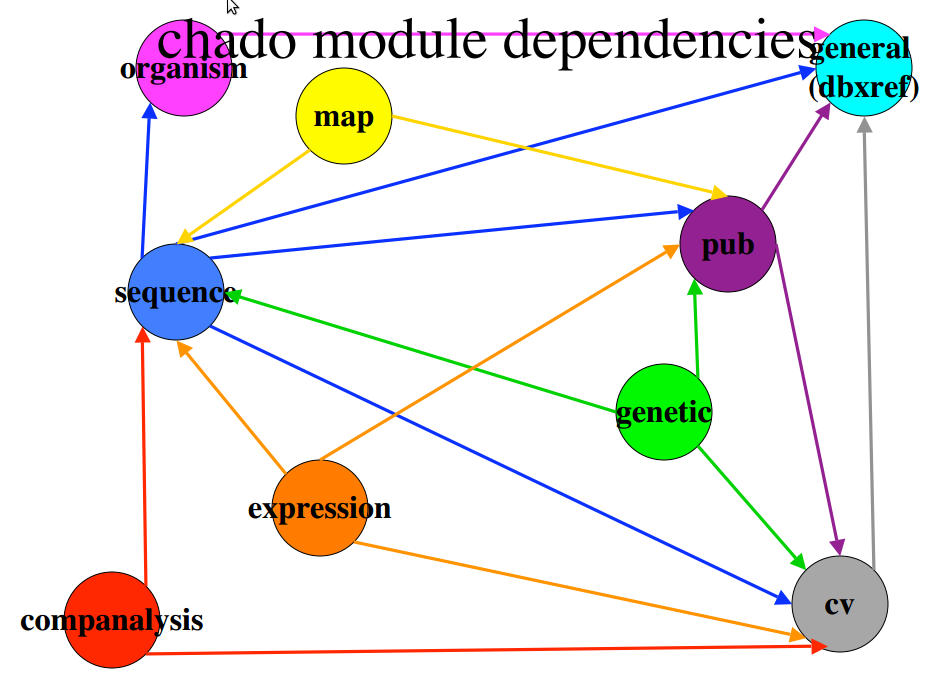
\includegraphics[height=110mm]{chado-dep.png}
\captionfonts
\caption[Chado Module Dependencies]{Graph of the dependencies between the Chado modules~\cite{chado_new}.}
\label{fig:chado-dep}
\end{center}
\end{figure}

\section{Example graph using the Chado genetics module}
The following figure depicts how ontologies are used in the Chado schema. This example uses the genetics module. In this example, the data being depicted is the Allele phenotype alpha-spec\textsuperscript{rg41}.
The ontology starts with the gcontext record which defines the gene. The gcontext record links to a phenstatement record which defines the phenotype class of the allele alpha-spec\textsuperscript{rg41}.
Specifically that the gene is lethal, larval, and recessive. All of the previous terminology link to separate cvterm records which define the common terminology used through the Chado schema.

\begin{figure}[h]
\begin{center}
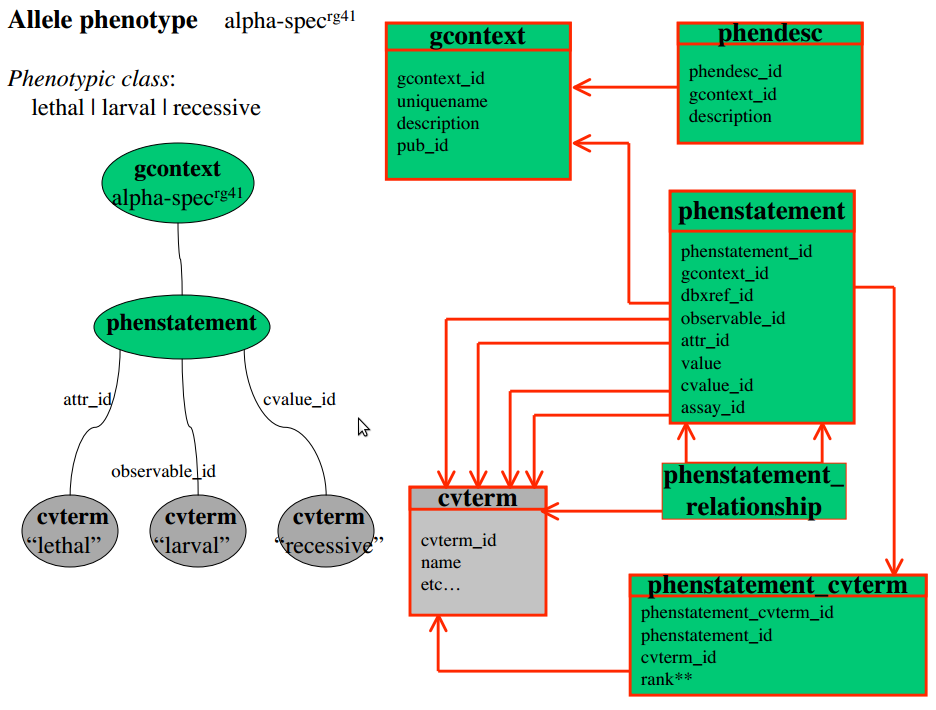
\includegraphics[height=110mm]{chado-ex.png}
\captionfonts
\caption[Chado Genetics Module Example]{Example Graph of Data in the Chado Genetics Module~\cite{chado_new}.}
\label{fig:chado-ex}
\end{center}
\end{figure}

\chapter{SQL create table statements for \textit{CGAT}}
\label{app:sql}
\begin{verbatim}
DROP TABLE IF EXISTS Users;
CREATE TABLE Users (
   UserId INT UNSIGNED NOT NULL AUTO_INCREMENT,
   FirstName VARCHAR(20) NOT NULL,
   LastName VARCHAR(40) NOT NULL,
   UserName VARCHAR(40) NOT NULL,
   Email VARCHAR(60) NOT NULL,
   Pass VARCHAR(64) NOT NULL,
   Salt VARCHAR(64) NOT NULL,
   LastLoginDate DATETIME NOT NULL,
   RegistrationDate DATETIME NOT NULL,
   Level INT NOT NULL,
   Role VARCHAR(10) NOT NULL,
   Exp INT NOT NULL,
   PRIMARY KEY ( UserId )
);

DROP TABLE IF EXISTS Groups;
CREATE TABLE Groups (
   GroupId INT UNSIGNED NOT NULL AUTO_INCREMENT,
   Name VARCHAR(80) NOT NULL,
   GroupDescription TEXT NOT NULL,
   CreateDate DATETIME NOT NULL,
   PRIMARY KEY ( GroupId )
);

DROP TABLE IF EXISTS Contigs;
CREATE TABLE Contigs (
   ContigId INT UNSIGNED NOT NULL AUTO_INCREMENT,
   Name VARCHAR(40) NOT NULL,
   Difficulty FLOAT NOT NULL,
   Sequence TEXT NOT NULL,
   UploaderId INT UNSIGNED NOT NULL,
   Source VARCHAR(20) NOT NULL,
   Species VARCHAR(100) NOT NULL,
   Status VARCHAR(20) NOT NULL,
   CreateDate DATETIME NOT NULL,
   PRIMARY KEY ( ContigId )
);

DROP TABLE IF EXISTS GroupMembership;
CREATE TABLE GroupMembership (
   GroupId INT UNSIGNED NOT NULL,
   UserId INT UNSIGNED NOT NULL,
   PRIMARY KEY ( GroupId, UserId )
);

DROP TABLE IF EXISTS Tasks;
CREATE TABLE Tasks (
   UserId INT UNSIGNED NOT NULL,
   ContigId INT UNSIGNED NOT NULL,
   Description TEXT NOT NULL,
   EndDate DATETIME NOT NULL,
   UNIQUE(UserId, ContigId),
   INDEX(UserId)
);

DROP TABLE IF EXISTS Annotations;
CREATE TABLE Annotations (
   AnnotationId INT UNSIGNED NOT NULL AUTO_INCREMENT,
   GeneId INT NOT NULL,
   StartPos INT UNSIGNED NOT NULL,
   EndPos INT UNSIGNED NOT NULL,
   ReverseComplement BOOL NOT NULL,
   PartialSubmission BOOL NOT NULL,
   ExpertSubmission BOOL NOT NULL,   
   ContigId INT UNSIGNED NOT NULL,
   UserId INT UNSIGNED NOT NULL,
   CreateDate DATETIME NOT NULL,
   LastModifiedDate DATETIME NOT NULL,
   FinishedDate DATETIME NOT NULL,
   Incorrect BOOL NOT NULL,
   ExpertIncorrect BOOL NOT NULL,
   ExpGained INT NOT NULL,
   PRIMARY KEY ( AnnotationId ),
   INDEX(UserId)
);

DROP TABLE IF EXISTS Exons;
CREATE TABLE Exons (
   ExonId INT UNSIGNED NOT NULL AUTO_INCREMENT,
   StartPos INT UNSIGNED NOT NULL,
   EndPos INT UNSIGNED NOT NULL,
   AnnotationId INT NOT NULL,
   PRIMARY KEY ( ExonId )
);

DROP TABLE IF EXISTS GeneNames;
CREATE TABLE GeneNames (
   GeneId INT NOT NULL AUTO_INCREMENT,
   Name VARCHAR(255) NOT NULL,
   PRIMARY KEY ( GeneId )
);


DROP TABLE IF EXISTS CollabAnnotations;
CREATE TABLE CollabAnnotations (
   CollabAnnotationId INT UNSIGNED NOT NULL AUTO_INCREMENT,
   GeneId INT NOT NULL,
   StartPos INT UNSIGNED NOT NULL,
   EndPos INT UNSIGNED NOT NULL,
   ReverseComplement BOOL NOT NULL,  
   ContigId INT UNSIGNED NOT NULL,
   CreateDate DATETIME NOT NULL,
   LastModifiedDate DATETIME NOT NULL,
   PRIMARY KEY ( CollabAnnotationId )
);

DROP TABLE IF EXISTS CollabExons;
CREATE TABLE CollabExons (
   ExonId INT UNSIGNED NOT NULL AUTO_INCREMENT,
   StartPos INT UNSIGNED NOT NULL,
   EndPos INT UNSIGNED NOT NULL,
   CollabAnnotationId INT NOT NULL,
   PRIMARY KEY ( ExonId )
);

DROP TABLE IF EXISTS ReadWriteTest;
CREATE TABLE ReadWriteTest(id INT, name VARCHAR(128));
\end{verbatim}

\end{document}